\documentclass[a4paper]{scrreprt}

% Uncomment to optimize for double-sided printing.
% \KOMAoptions{twoside}

% Set binding correction manually, if known.
% \KOMAoptions{BCOR=2cm}

% Localization options
\usepackage[english]{babel}
\usepackage[T1]{fontenc}
\usepackage[utf8]{inputenc}

% Quotations
\usepackage{dirtytalk}

% Floats
\usepackage{float}

% Enhanced verbatim sections. We're mainly interested in
% \verbatiminput though.
\usepackage{verbatim}

% Automatically remove leading whitespace in lstlisting
\usepackage{lstautogobble}

% CSV to tables
\usepackage{csvsimple}

% PDF-compatible landscape mode.
% Makes PDF viewers show the page rotated by 90°.
\usepackage{pdflscape}

% Advanced tables
\usepackage{array}
\usepackage{tabularx}
\usepackage{longtable}

% Fancy tablerules
\usepackage{booktabs}

% Graphics
\usepackage{graphicx}

% Current time
\usepackage[useregional=numeric]{datetime2}

% Float barriers.
% Automatically add a FloatBarrier to each \section
\usepackage[section]{placeins}

% Custom header and footer
\usepackage{fancyhdr}

\usepackage{geometry}
\usepackage{layout}

% Math tools
\usepackage{mathtools}
% Math symbols
\usepackage{amsmath,amsfonts,amssymb}
\usepackage{amsthm}
% General symbols
\usepackage{stmaryrd}

% Utilities for quotations
\usepackage{csquotes}

% Bibliography
\usepackage[
  style=alphabetic,
  backend=biber, % Default backend, just listed for completness
  sorting=ynt % Sort by year, name, title
]{biblatex}
\addbibresource{references.bib}

\DeclarePairedDelimiter\abs{\lvert}{\rvert}
\DeclarePairedDelimiter\floor{\lfloor}{\rfloor}

% Bullet point
\newcommand{\tabitem}{~~\llap{\textbullet}~~}

\pagestyle{plain}
% \fancyhf{}
% \lhead{}
% \lfoot{}
% \rfoot{}
% 
% Source code & highlighting
\usepackage{listings}

% SI units
\usepackage[binary-units=true]{siunitx}
\DeclareSIUnit\cycles{cycles}

\newcommand{\lecture}{41109 - Privacy and Data Security}
\newcommand{\series}{06}
% Convenience commands
\newcommand{\mailsubject}{\lecture - Series \series}
\newcommand{\maillink}[1]{\href{mailto:#1?subject=\mailsubject}
                               {#1}}

% Should use this command wherever the print date is mentioned.
\newcommand{\printdate}{\today}

\subject{\lecture}
\title{Series \series}

\author{Michael Senn \maillink{michael.senn@students.unibe.ch} --- 16-126-880}

\date{\printdate}

% Needs to be the last command in the preamble, for one reason or
% another. 
\usepackage{hyperref}

\begin{document}
\maketitle


\setcounter{chapter}{\numexpr \series - 1 \relax}

\chapter{Series \series}

\section{\emph{k}-anonymity and \emph{l}-diversity}

Let $A$ be a dataset sanitized with discrete \emph{l}-diversity. Then, every
equivalence class $C$ contains at least $l$ distinct combinations of sensitive
attributes. As such $C$ contains at least $l$ rows, and hence has
\emph{l}-anonymity.

Similarly let $A$ be a dataset sanitized with probabilistic \emph{l}-diversity.
Then for every equivalence class $C$, every combination of secret attribute
values $(s1, \ldots, s_n)$ contained in $C$ makes up at most a fraction of
$l^{-1}$ of the equivalence class. Any such equivalence class $C$ will thus
have at least $l$ combinations of different sensitive information, each
accounting for $l^{-1}$ of the equivalence class. As such it has distinct
\emph{l}-diversity, and per above also also \emph{l}-anonymity.

\section{Implementing \emph{k}-anonymity with the Mondrian algorithm}

\subsection{NCP as a fucntion of \emph{k}-anonymity}

The provided implementation of the Mondrian algorithm was used to sanitze the
sample dataset to various levels of \emph{k}-anonymity. The achieved ``NCP''
--- a measure of how generalized the data is, in the range of $[0, 1]$  ---
plotted versus the $k$ parameter is shown in figure \ref{fig:k_anonymity_ncp}.

\begin{figure}
		\centering
		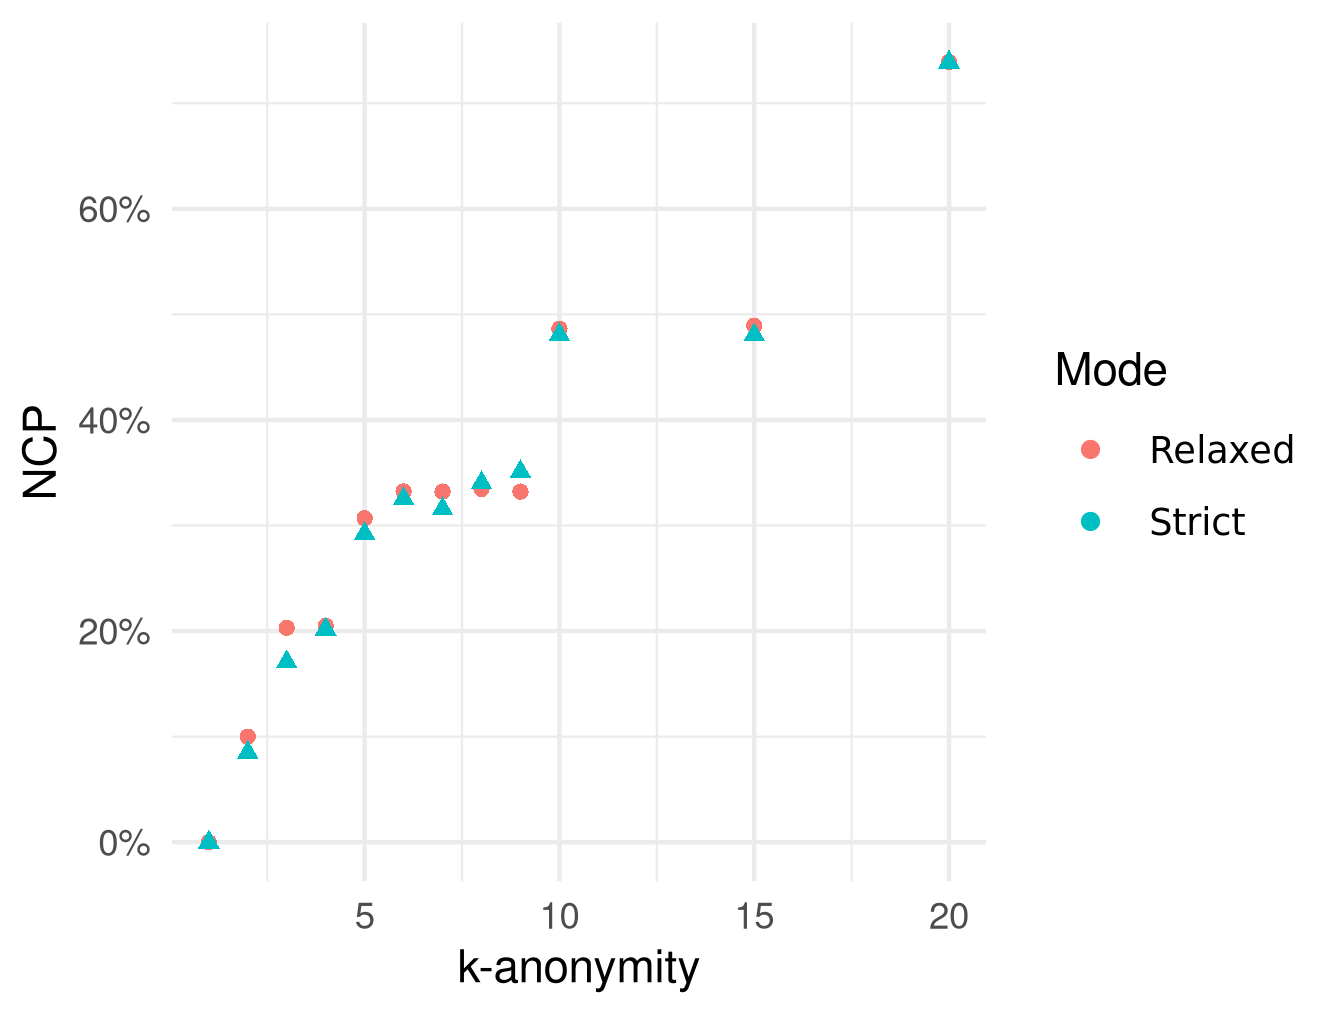
\includegraphics[width=\textwidth]{resources/k_anonymity_ncp.png}
		\caption{NCP as a function of \emph{k}-anonymity}
		\label{fig:k_anonymity_ncp}
\end{figure}

As expected the degree of generalization which is required goes up the higher
$k$ is. For 3-anonymity it is around \SI{20}{\percent}, for
5-anonymity around \SI{30}{\percent}, for 10-anonymity around
\SI{50}{\percent} and for 74-anonymity --- $74$ being the size of the
full dataset --- \SI{100}{\percent}.

No meaningful difference is visible between strict and relaxed mode of the
Mondrian algorithm.

\subsection{Improving the algorithm with randomization}

As the algorithm is greedy, its outcome will be influenced by the ordering of
data. As such it can be optimized by running it multiple times over
permutations of the input data, keeping the \emph{k}-anonymization with the
lowest NCP value.

As the provided implementation is a mess, with global state preventing
successful subsequent executions of the algorithm, this was measured by means
of a separte Python program which invokes the anonymizer multiple times in
sequence, shuffling its input file inbetween invocations.

Figure \ref{fig:k_anonymity_ncp_randomized} shows that, with 100 attempts each,
marginally lower NCP values can be achieved --- albeit at the cost of
significantly increasing the time anonymization takes. Improvements were in the
range of \SIrange{2}{5}{\percent}.

\begin{figure}
		\centering
		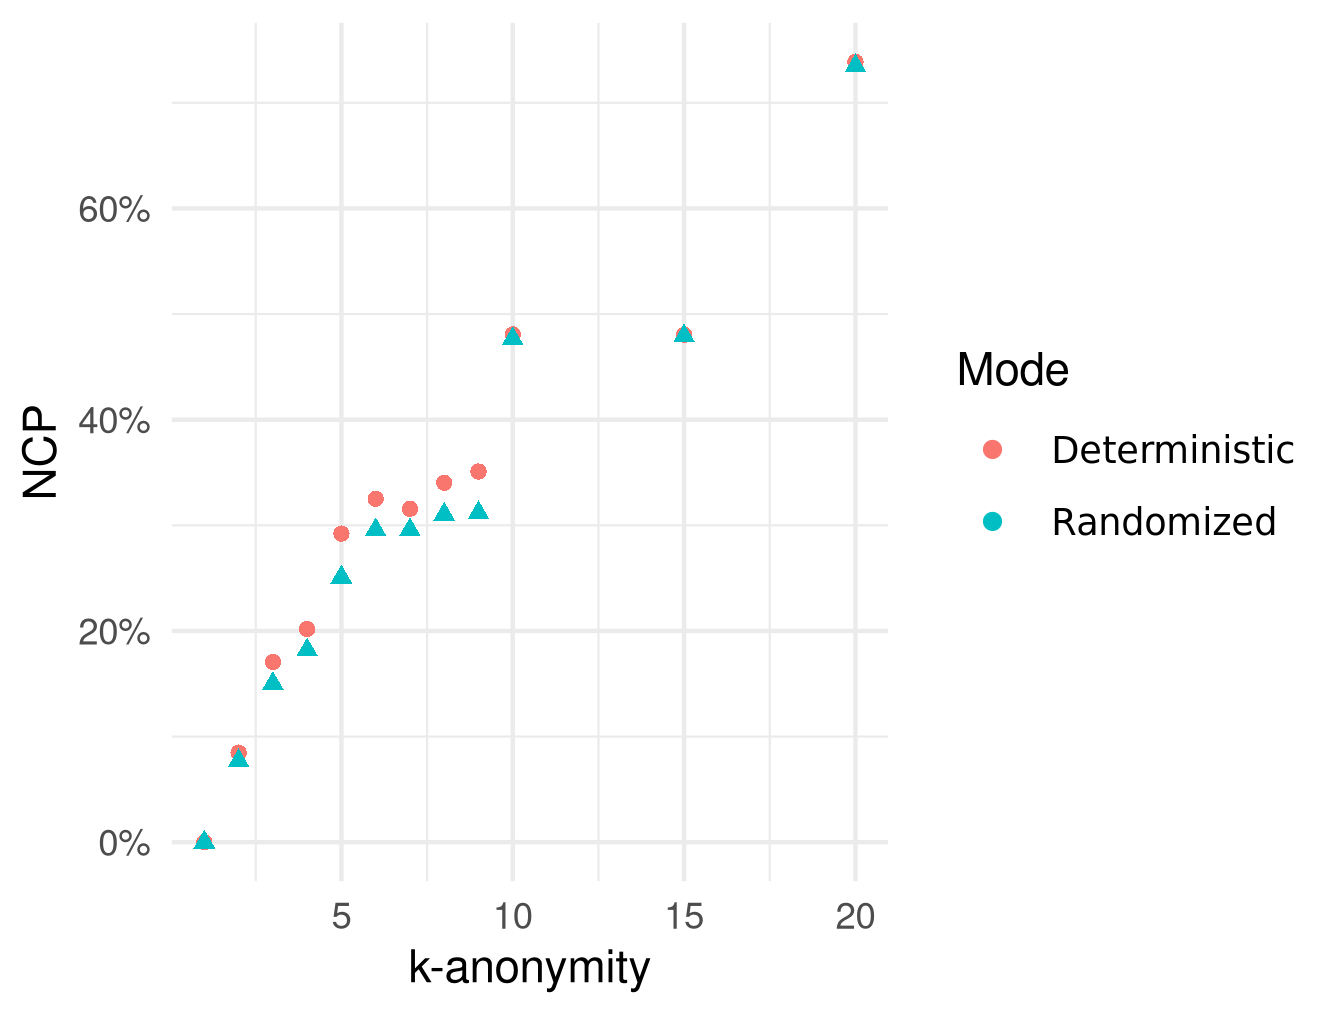
\includegraphics[width=\textwidth]{resources/k_anonymity_ncp_randomized.png}
		\caption{NCP as a function of \emph{k}-anonymity, optimized with randomization}
		\label{fig:k_anonymity_ncp_randomized}
\end{figure}

\printbibliography

\end{document}
